\documentclass[conference]{IEEEtran}
\IEEEoverridecommandlockouts{}
% The preceding line is only needed to identify funding in the first footnote. If that is unneeded, please comment it out.
\usepackage{cite}
\renewcommand{\citepunct}{,\penalty\citepunctpenalty\,}
\usepackage{amsmath,amssymb,amsfonts}
\usepackage{algorithmic}
\usepackage{graphicx}
\usepackage{booktabs}
\usepackage{textcomp}
\usepackage{xcolor}
\usepackage{footnote}
\usepackage{url}
\usepackage{hyperref}
\usepackage{subcaption}               % subfiguren
\usepackage{scrextend}

\def\BibTeX{{\rm B\kern-.05em{\sc i\kern-.025em b}\kern-.08em
\kern-.1667em\lower.7ex\hbox{E}\kern-.125emX}}

% URL's bibliography overflow prevention
\def\UrlBreaks{\do\/\do-}
% \setlength{\parskip}{8pt}

\begin{document}
\title{\textbf{\LARGE Time Is Running Out\\
        \large Assessing Temporal Privacy of Privacy Zones in Fitness Tracking Social Networks}
}

\author{
    \IEEEauthorblockN{Deleu, Wout}
    \IEEEauthorblockA{
        \textit{KU Leuven, Campus Rabot} \\
        Ghent, Belgium
    }
}
\maketitle
\thispagestyle{plain}
\pagestyle{plain}

\begin{abstract}
    In a society where social media is so ubiquitous, the privacy concerns
    around them are more relevant than ever.  During this article, the main
    focus will be on the privacy policies of fitness trackers. Fitness trackers are
    platforms which store and display data related to sport activities. These can
    be shared with other users. This data may include heart rate, GPS-locations,
    etc. This type of data sharing can however cause unintentionally sharing of
    sensitive information, like home addresses.

    Most fitness tracking networks are aware of this danger and implement a series
    of countermeasures to prevent this. One of these countermeasures is the use of
    Endpoint Privacy Zones (EPZs) which is a zone around a sensitive location,
    which hides the part of the trajectory which ends or begins in this zone.
    Previous research has shown that it is possible to retrieve the sensitive
    location using the available data from the activity. Dhondt et al.\ showed that
    based on the total distance travelled, the sensitive location can be retrieved
    using an `inference attack'~\cite{Dhondt}. This study will investigate the
    possibilities of such inference attacks using other data than the distance. We
    want to recreate the results as good as possible using the speed and tempo of
    the activity, together with GPS-locations. This can result in an attack model
    with a success rate up to 75\%. This is lower than the previous implementation
    of Dhondt et al., but this shows that the attack is still possible under
    circumstances where the distance is rendered unusable. This also includes some
    countermeasure described by Dhondt et al. But countermeasures like enlarging
    the EPZ or shifting endpoints still have effect.\vspace{6pt}

\end{abstract}
\begin{IEEEkeywords}
    fitness-trackers, privacy, GPS-locations, endpoint privacy zone, inference attack
\end{IEEEkeywords}

\section{\textbf{Introduction}}
Social media has become virtually indispensable in today's modern life and
branches out into a lot of facets, including social networking, media sharing
networks, etc, but also the branch of fitness trackers. This rise of these new
media, however, also brings unintended but significant privacy concerns.

The focus of this thesis is on privacy within these fitness trackers, more
specific platforms that use GPS locations, such as
Strava\footnote{\label{fn:strava}\url{https://www.strava.com/}}, Nike Run Club,
etc. These are platforms where individuals can share sports activities such as
running, cycling, hiking, \ldots with each other. The general concept is here
that when you perform a sports activity, you make it available to your
followers and friends. The sports activities will naturally release certain
data to those other users, which could possibly have negative effects on the
users privacy. For example leaking the home address of the user, which can lead
to stalking and burglary~\cite{Sportapp72:online, Cyclistw89:online}. There are
even some reports about military bases being discovered using the Strava
heatmap~\cite{Fitnesst33:online}.
\begin{figure}[h]
    \centering
    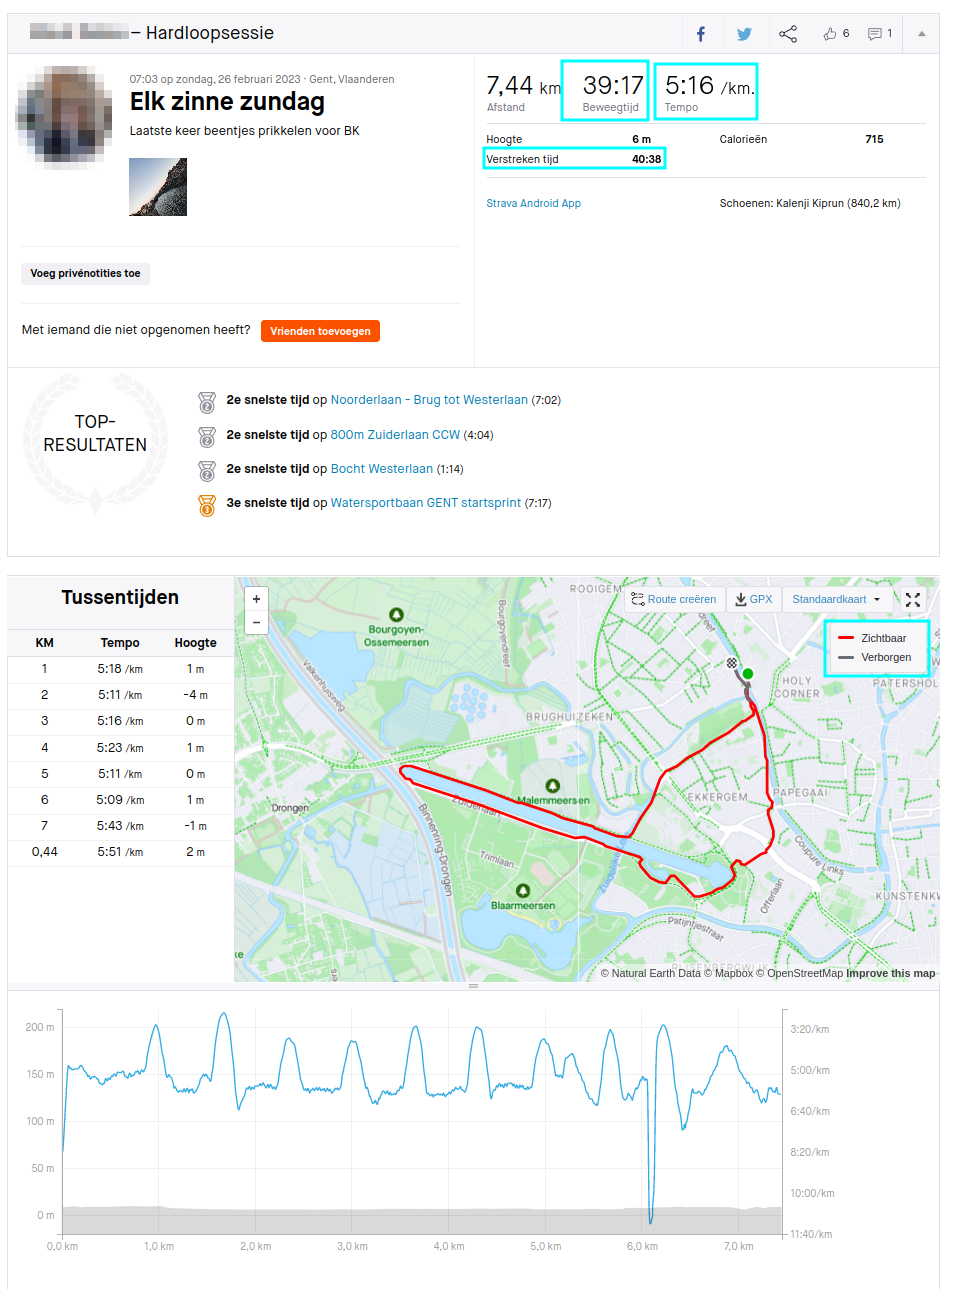
\includegraphics[width=\linewidth]{fig/VoorbeeldActiviteiten/VoorbeeldActiviteit_Personal.png}
    \caption{Example of a Strava activity}\label{fig:activity}
\end{figure}

Fitness trackers each implement ways to improve user privacy. Perhaps the most
easy way to think of is perhaps the ability to hide activities from a selection
of people (e.g., anyone who is not a follower). Thus, only the people whom the
user explicitly allows to view activities. A more complex alternative is to use
EPZs. Hereby a portion of the displayed route will be hidden for external
viewers. Part of the route is cut off, so to speak. The real starting and
ending points will lie inside the truncated part. New points will be generated,
on the edge of the circle, which for the external observer will represent the
beginning and end. The beginning and end part of the route will thus become
invisible to the other users. Due to the presence of all these attempts at
privacy enhancements, it is noticeable that the developers of the platforms are
very aware of the potential dangers. However, there is a trade-off to be made
when implementing between the usability of the platform, and the privacy of the
end user. The more data is released, the greater the chance of potentially
sensitive info being passed along. On the other hand, when omitting
information, the usability and presence of useful data of the platform is
greatly diminished.

In this study, we consider whether there is a possibility to retrieve hidden
locations of an activity, despite the use of an EPZ as privacy security
mechanism. Some ways to bypass the EPZ using other metadata such as elevation
data and distances have been described in the past~\cite{Verdonck_2022, Dhondt,
    sec18has3:online}. This thesis goes into more detail on the use of velocity
data. As a base for this attack, we use the inference attack, which was
described by Dhondt et al. We investigate whether this attack is still possible
when omitting certain data, and thus by the use of alternative data. The focus
of this study is mainly on velocity-based data.

To achieve this objective, we must first examine the attack model according to
Dhondt et al. Then we can describe different possible alternative attack
scenarios, and for each work out the calculations necessary in order for this
scenario to be possible. Before we can test and analyze the attack, we must
consider the possible errors in the used dataset. We also perform an analysis
on the difference between the calculated distances, and the values derived
according to the calculations of Dhondt et al. So can we estimate the
effectiveness of the attack a priori to some extent. Only then do we execute
the attack, evaluate the attacks and form meaningful conclusions.

\section{\textbf{Background}}
\subsection{Fitness Trackers}
The data used to test the effectiveness the attack and perform experiments
comes from the popular fitness tracker Strava\footref{fn:strava}. This is a
social network where all types of athletes can share their activities. This
includes running, walking, cycling, swimming, \ldots The collected data is
filtered according to the perspective of a possible attacker. Not all data
turns out to be useful. Only data that could reveal sensitive information
regarding residence is retained. This will therefore mean that only activities
that contain relevant GPS information will be considered, so only
\textit{runs}, \textit{hikes}, \textit{walks}, and \textit{bike rides}.
\begin{figure}[h]
    \centering
    
\includegraphics[width=0.6\linewidth]{fig/Logo_Strava.png}
    \caption{Strava logo~\cite{strava_companie}}\label{fig:stravalogo}
\end{figure}

\subsection{GPS faults}
Some visible data of an activity, which can also be found on
Figure~\ref{fig:activity}, are distance, duration, average speed, etc. The
average speed forms the core to the attack which we will describe in this
article. This will be calculated as the total distance divided by the moving
time of the athlete. Fitness trackers receive raw data from the devices. This
data must therefore be processed before it is usefull fo the users. Especially
GPS-data, which can be exposed to a lot of faults and noise. There are three
types of GPS faults, namely \textit{GPS drift}, \textit{GPS signal loss} and
\textit{GPS bounce}. GPS-drift is a phenomenon where a user's GPS location
deviates from the effective location. This may be caused by densely built
environments, and natural factors such as tall trees. GPS bouncing is an
anomaly caused mainly by tall buildings. In this situation, the GPS signal will
bounce in between buildings on its way to the device from the satellite. The
extra delay that the bounces bring along causes the device to mistakenly think
it has traveled some additional distance. The outcome of the trajectory is then
unpredictable, leading to a `cluster' of GPS points. A last incident that can
occur is GPS signal loss. This occurs when the user's signal is lost, and a new
signal is only received at a later time stamp, causing a jump. A second cause
that can lead to signal loss, which especially applies to fitness trackers, is
the ability to pause an activity. When the activity is resumed again, there
will be a jump in GPS locations, which may lead to miscalculation of distance.

\begin{figure}[h]
    \centering
    \begin{subfigure}[b]{.48\linewidth}
        \centering
        \caption{GPS bounce example}
        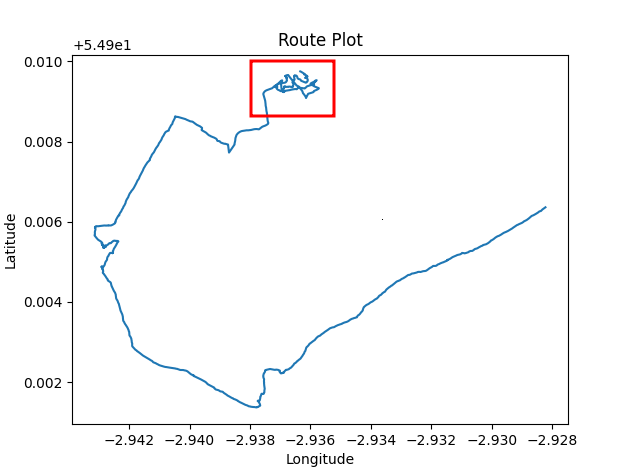
\includegraphics[width=\linewidth]{fig/Afwijkingen&Analyses/Crooked Routes/Crooked GPS Route_Cart.png}
    \end{subfigure}
    \begin{subfigure}[b]{.38\linewidth}
        \centering
        \caption{GPS signal loss}
        \includegraphics[width=1\linewidth]{fig/Afwijkingen&Analyses/Crooked Routes/1_Full_withArrow.png}
    \end{subfigure}
    \begin{subfigure}[b]{0.75\linewidth}
        \centering
        \caption{GPS drift}
        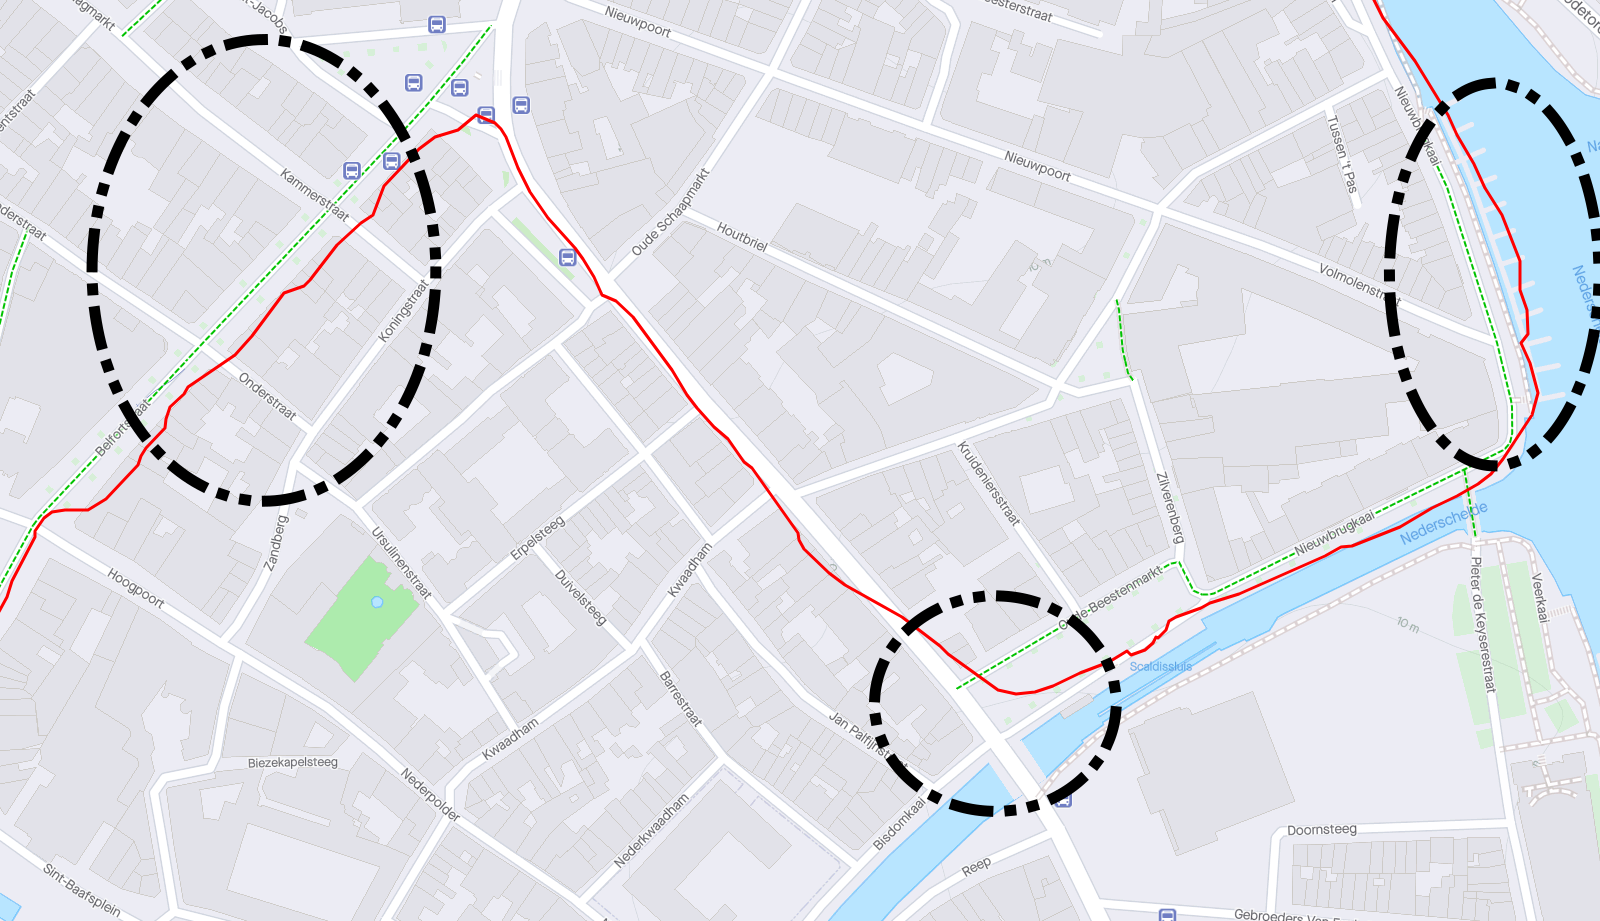
\includegraphics[width=\linewidth]{fig/Afwijkingen&Analyses/Crooked Routes/GPS-Drift.png}
    \end{subfigure}
    \caption{Possible GPS-faults}
\end{figure}

Some techniques can be used to improve the overall accuracy of the GPS data,
and so improve the effectiveness of the attack. The main technique used in this
thesis is \textit{smoothing}, and the hypothesis is that fitnessplatforms use
this technique as well. This is a technique to enhance the accuracy and
reliability of GPS data. There are different implementations of GPS smoothing,
but the one used in this context is moving average filtering. This method
calculates an average position by considering a sliding window of the most
recent GPS measurements. By averaging multiple measurements over a certain time
period, the effects of noise and temporary inaccuracies can be mitigated,
resulting in a smoother and more reliable trajectory. The size of the window
can be chosen. The larger the window, the less accurate the trajectory will be,
but the more noise will be countered. This technique is especially useful to
counter GPS bouncing and GPS drift.

\subsection{Endpoint Privacy Zones}
An important privacy-enhancing mechanism is the use of an \textit{Endpoint
    Privacy Zone} (EPZs). An EPZ is a circular zone with a certain radius around a
GPS point, which represents a sensitive location. The radius of this circle can
be chosen by the user. In the case of Strava, users have the option to select
values ranging from 0 to 1600m, in increments of 200m. When a user starts or
finishes their activity within this zone, that specific part of the route
within the EPZ will not be visible to others. From another user's perspective,
the activity will appear to start and/or end at the edge of this circle (which,
of course, is not visible). It's important to note that if a user passes
through the EPZ without stopping within it, that segment of the route remains
unmodified.
\begin{figure}[h]
    \centering
    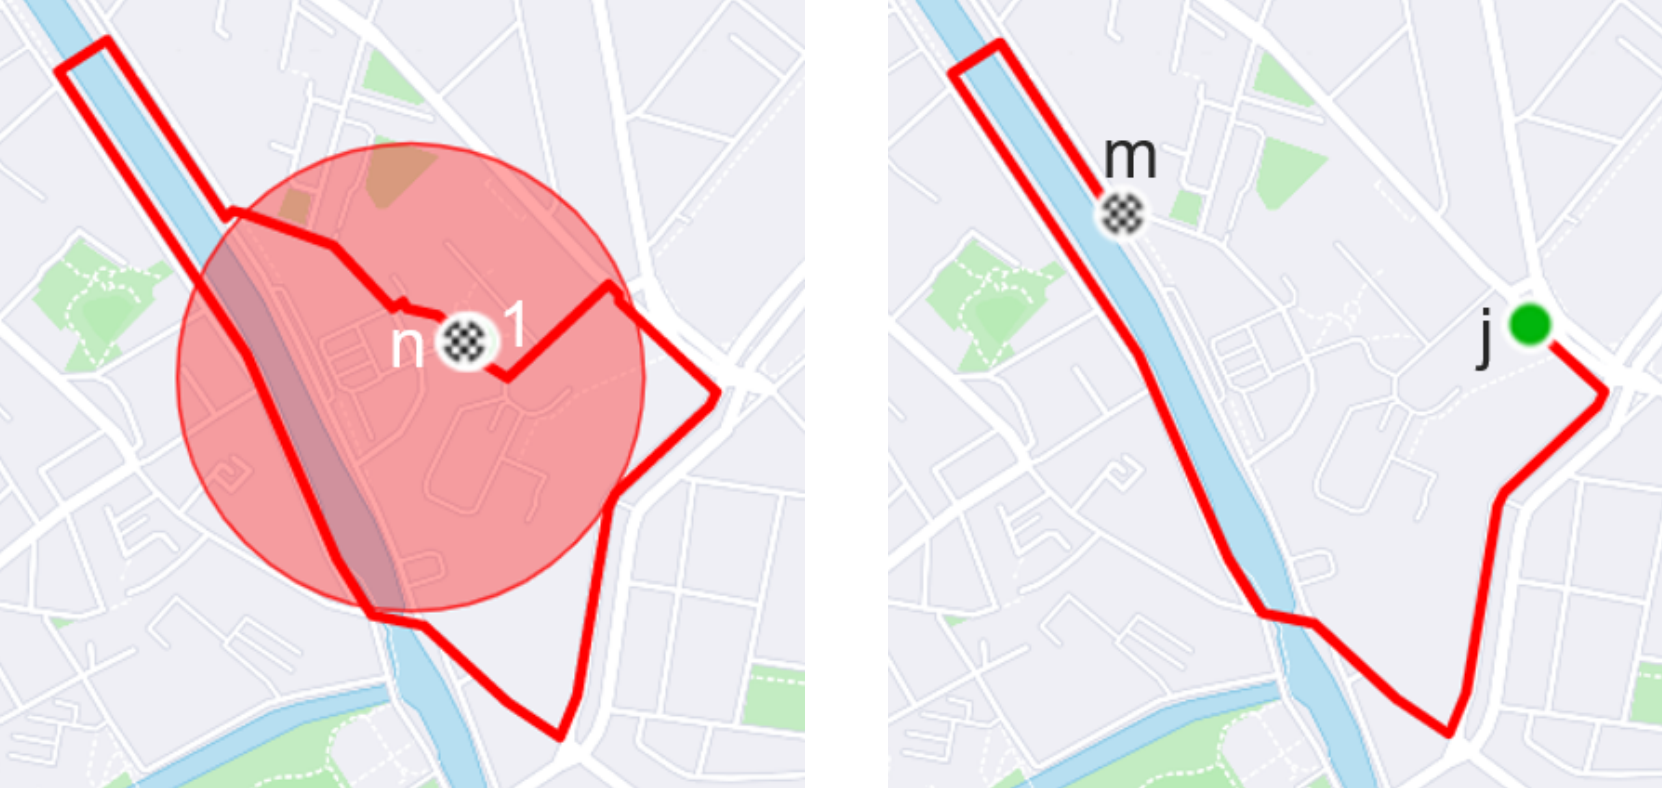
\includegraphics[width=\linewidth]{fig/EPZ-mechanisme/DropEPZPoints.png}
    \caption{Example EPZ filtering mechanism~\cite{Dhondt}}\label{fig:epzmechanisme}
\end{figure}

\subsection{Related work}
There has been previous research conducted on the effectiveness of EPZs in
fitness trackers. Hassan et al. (2018) presented an implementation of EPZs
where the sensitive location serves as the center of the
zone~\cite{sec18has3:online}. This means that in this scenario by identifying
this zone, one can determine the sensitive location. However, in contrast to
most real world implementations of EPZs, it is assumed that the center does not
undergo any translation, and therefore no spatial cloaking is applied. Dhondt
et al. (2022) also conducted a study on potential vulnerabilities in the
concept of EPZs~\cite{Dhondt}. The paper places particular emphasis on the
translation of the EPZ and its impact on user privacy. It introduces an
inference attack that exploits the total distance covered in an activity. In
brief, the attack operates as follows: by leveraging the total distance
traveled and combining it with the road network in the given environment, an
attempt is made to reconstruct all possible routes that the athlete could have
taken. This analysis is performed for each activity. By comparing these
reconstructed routes, it becomes possible to predict a location that is deemed
most likely to be the sensitive location.

\section{\textbf{Setting of the attack}}
\subsection{Threat model}
This thesis focuses the feasibility of bypassing EPZs from the perspective of
an attacker, who is a user of the platform without ownership of the activity
data. Given that activities are cloaked using EPZs, the attacker lacks
visibility into the actual start and/or end locations. Consequently, their
objective is to determine the sensitive location despite the presence of
cloaking. It is important to note that the attacker in this thesis does not
have access to assistance data or state data. However, they do have access to
raw GPS data, as well as additional information such as speed and pace.

The research aims to explore the extent to which an attack is still possible
when the distance data is rendered unusable. Therefore, an alternative approach
to the inference attack is investigated to determine its potential success. The
thesis presents a theoretical framework to describe the attacker and examines
the circumstances under which the attack remains feasible, as well as effective
countermeasures. The overall scenario assumed is: what if fitness trackers were
to obfuscate or make the distance data unusable through techniques like
rounding or adding uncertainty? In such a case, would the attack still be
possible? If so, what would be its effectiveness and how would it impact the
previously discussed protective measures?

To enable the attack, certain assumptions need to be made. The first assumption
is that the visible start and end points must lie on the edge of the EPZ
circle~\cite{Dhondt}. Secondly, the protected location, which is the sensitive
location, must be located on the road graph. It cannot be outside the mapped
area, such as in a forest where there are no paths. The user is expected to
follow the shortest route within the EPZ.\ Additionally, this thesis relies on
average speeds and paces, leading to the proposal of an additional assumption:
the user should not remain stationary within the EPZ.\ Lastly, it is assumed
that activities that involve two concealed locations, such as both start and
endpoints being hidden, are not usable for the purposes of this thesis.

\subsection{Inference Attack}
The actual attack can be broken down in seven steps.
\begin{enumerate}
    \item The first step is to identify the EPZ, which, although not mandatory,
          significantly narrows down the search space. In this process, all the
          activities made available by a user are considered. The visible start and end
          points of these activities are extracted and then grouped together using the
          k-means algorithm. This grouping helps to form a circle that represents the
          EPZ.\
    \item Then we can move on to the identification of Entry Gates (E.G.). Entry gates
          refer to the zones where users can enter or exit the EPZ.\ These gates are
          typically located around roads that lead into the EPZ.\ Identifying these entry
          gates is crucial for filtering out anomalous activities. The detection of entry
          gates is accomplished using the Density-Based Spatial Clustering of
          Applications with Noise (DBSCAN) algorithm.
    \item For each identified EPZ, it is necessary to create a graph representation of
          the surrounding area. The graph representation consists of a series of nodes,
          all located on a known street. The edges connecting the nodes follow the street
          layout, representing possible routes~\cite{neira2022graph}. Based on the nodes
          in this graph, the Distance Matrix can be constructed. This matrix contains the
          theoretical distances from all starting nodes (on the boundary of the EPZ) to
          all nodes present in the graph. By utilizing the Dijkstra algorithm, it becomes
          possible to determine the shortest theoretical distance from each point to all
          other points in the graph. These distances are stored and are crucial in the
          later stages of the attack.
    \item To make an effective prediction, it is crucial to know the distance traveled
          within the EPZ.\ This is referred to as the inner distance. Two possible
          scenarios apply in this thesis: one where the cumulative distance is known,
          from which we can infer the distance traveled outside the EPZ, and another
          where this distance is unknown. In the first scenario, the conversion is
          performed using the following equation: $inner\ distance = total\ time \times
              average\ speed - outer\ distance \label{eq:inner}$. However, if the distance is
          unknown, the outer distance needs to be calculated externally using visible GPS
          locations. The outer distance utilizes the Haversine formula to calculate
          distances between two points on a spherical
          surface~\cite{sheppard1922practical}.
    \item Prior to predicting the location, it is important to filter out activities that
          cannot yield useful predictions. We aim to exclude all other activities as much
          as possible. In cases where a user does not follow the shortest route from the
          EPZ boundary to the sensitive location, we can partially address this by
          considering an activity only if the remaining distance within the EPZ is
          smaller than the maximal possible distance to be covered. Similarly, filtering
          can be applied for distances traveled that are lower than the minimum possible
          distance. Furthermore, the visible start and end points of activities are
          checked for compatibility with the road graph. If the difference in distance
          between the original location and the snapped location is too large, the
          activity is filtered out. Lastly, deviations in the E.G. are examined. If there
          is a deviation between the visible start and end points and the E.G. that
          exceeds three times the standard deviation, the activity is filtered out.
    \item The next step is to predict the sensitive location. To make a prediction for
          each activity, the calculated inner distance is used. This inner distance is
          then matched with the street network. The idea behind this is to traverse all
          possible routes (forming the shortest path to the nodes on the path) within the
          EPZ and stop when the traveled distance matches the calculated inner distance.
    \item To transform the routes determined in the previous step into a final
          prediction, regression analysis is applied using the Least Absolute Deviations
          (LAD) method. The outcome of this regression analysis will be a GPS location,
          which will form our final prediction.
\end{enumerate}
Note that this attack is very similar to the attack proposed by Dhondt et al.\ and Verdonck T.~\cite{Dhondt,Verdonck_2022}.

\section{\textbf{Used Data}}
It is crucial to use a representative dataset in order to draw meaningful
conclusions and identify potential deviations or irregularities. By examining
the characteristics of the data, we can form well-grounded conclusions that
take into account certain properties of the data. Since this thesis builds upon
the research of Dhondt et al., it is convenient to continue working with their
dataset. In total, a dataset of 4000 users was collected. However, this thesis
only experiments with a subset of 131 users, with 101 users used for analyses
and conclusions, and 30 users reserved for testing the attack.

\subsection{Geographical distribution}
A geographical distribution is visible in Figure~\ref{fig:heatmap}. It clearly
shows that most activities are located in Central Europe. Additionally, there
is a noticeable concentration in the United States. To a lesser extent, there
are also activities in Australia and South America. The dataset exhibits a
relatively broad spread of activities worldwide, providing a solid foundation
for testing the attack. However, it is important to note that the fraction of
the dataset we have access to, with 101 users, is relatively small, which may
result in a distorted representation of reality.
\begin{figure}[h]
    \centering
    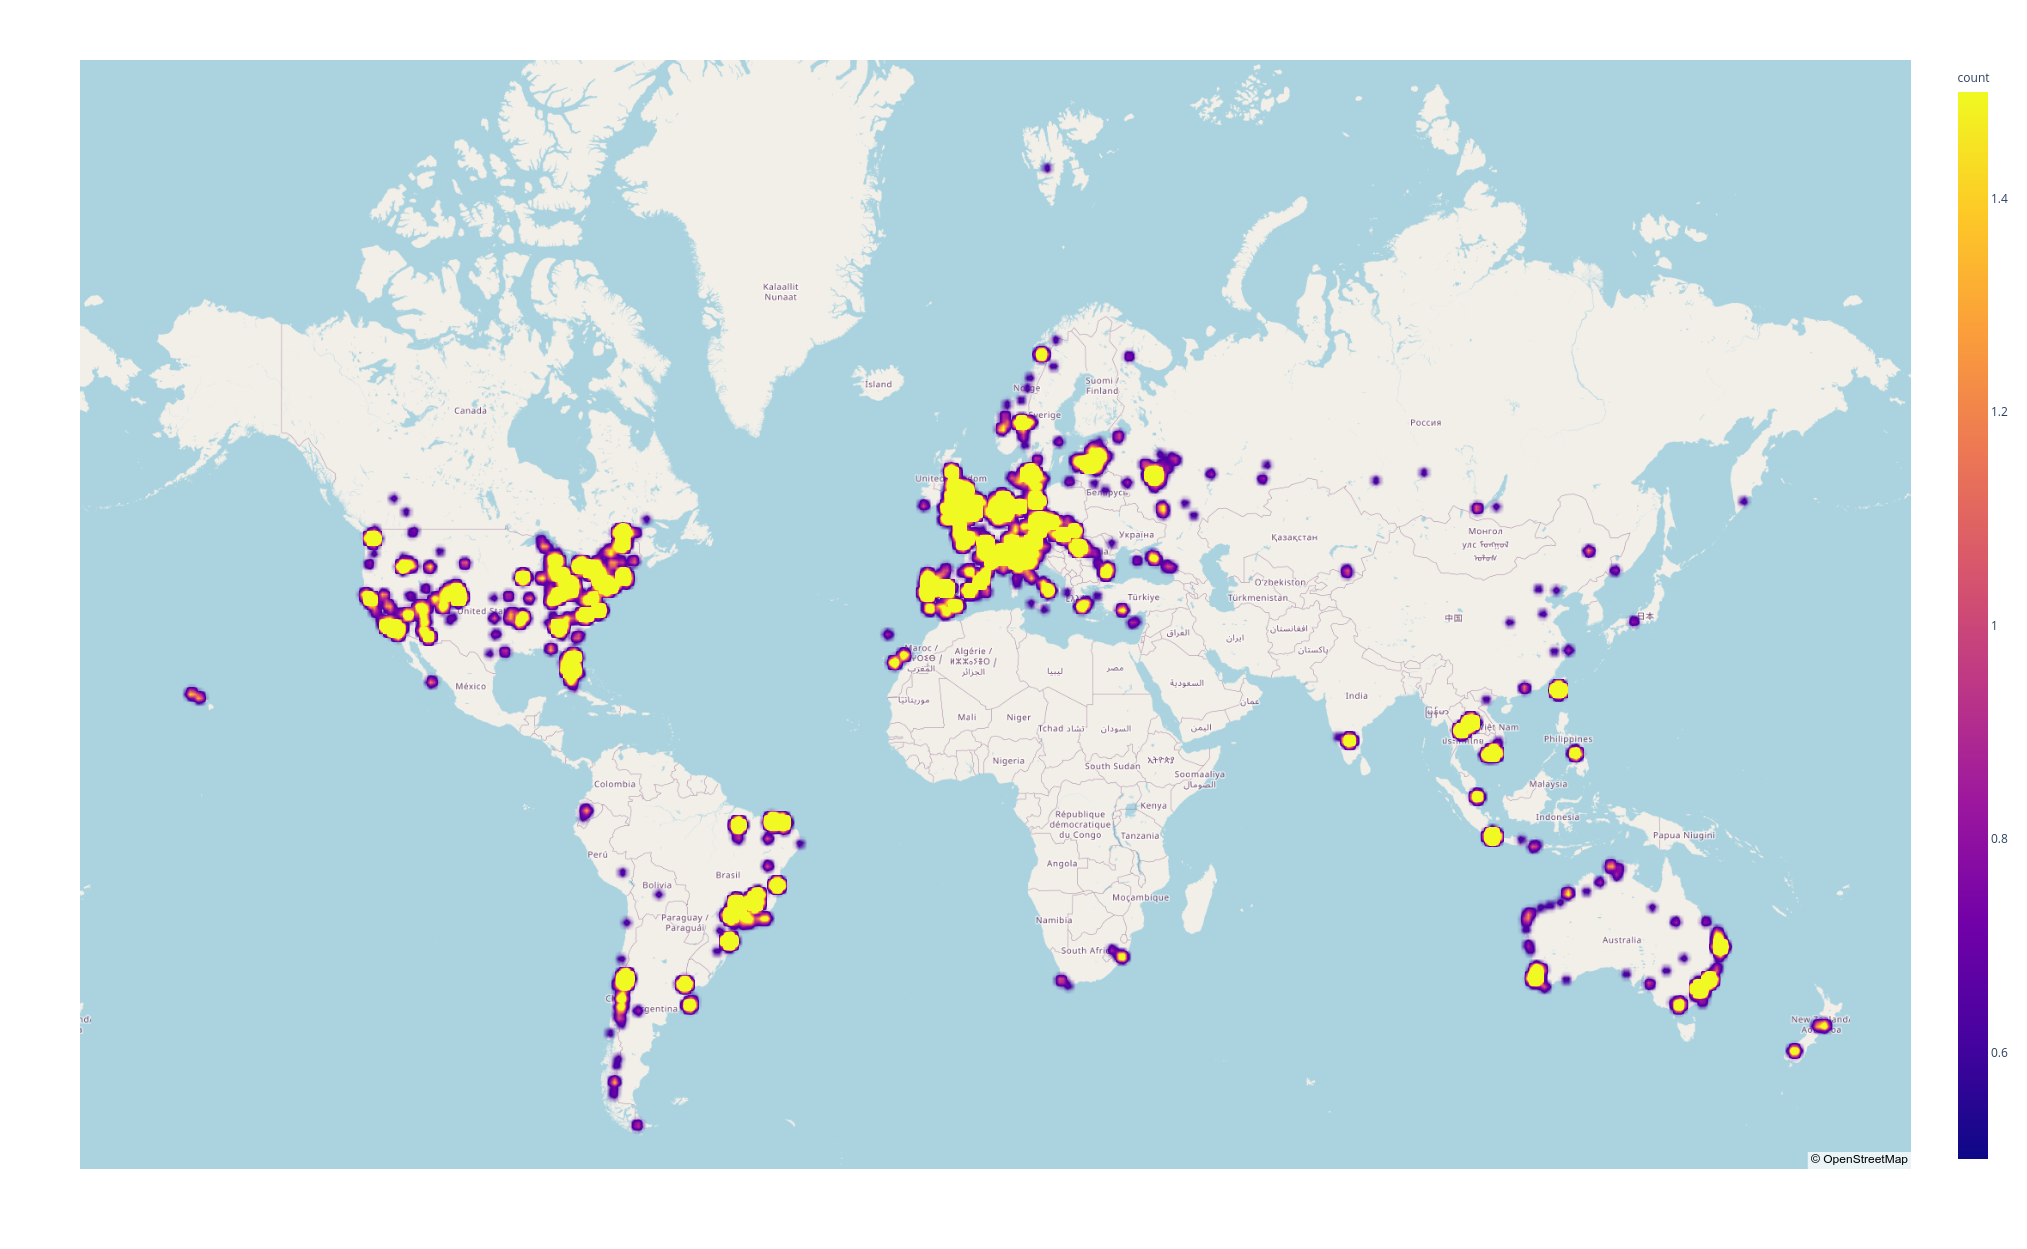
\includegraphics[width=0.85\linewidth]{fig/Afwijkingen&Analyses/Heatmap.png}
    \caption{Geo-heatmap of the users in the dataset}\label{fig:heatmap}
\end{figure}

\subsection{Users and activities}
Table~\ref{tab:stats_dataset} displays several global statistics regarding
users and their associated activities in the dataset. Figure
~\ref{fig:cdf_amount_activities} shows the CDF plot, illustrating the number of
activities per user. It is notable that there is a significant number of
activities available per user in the dataset. However, it's important to note
that the dataset, with an average of 411 activities per user, is not entirely
representative of reality. When comparing these figures with data from a study
conducted by Strava itself in 2020, there seems to be a mismatch.
\begin{table}[h]
    \centering
    \begin{tabular}{|l||c|}
        \hline
                                             & \textbf{Amount} \\
        \hline \hline
        Total \# users                       & 101             \\
        \hline
        Total \# activities                  & 41 554          \\
        \hline
        Average \# activities per user       & 411             \\
        \hline
        Median of the \# activities per user & 296             \\
        \hline
        Maximal \# activities for a user     & 2946            \\
        \hline
        Minimaal \# activities for a user    & 31              \\
        \hline
    \end{tabular}
    \captionsetup{justification=centering}
    \caption{Overview of users and activities}\label{tab:stats_dataset}
\end{table}
\begin{figure}[h]
    \centering
    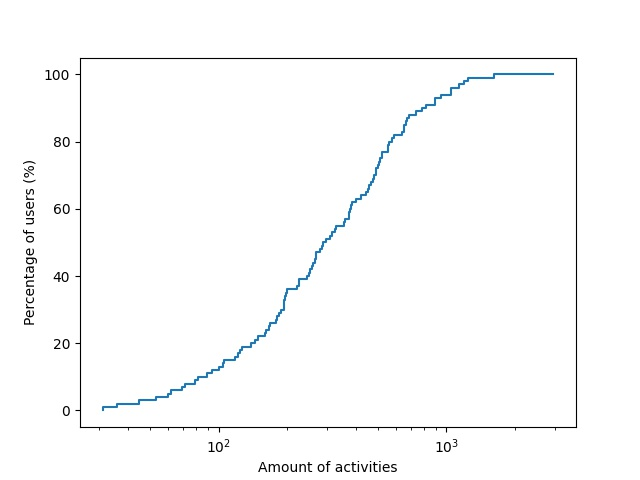
\includegraphics[width=0.8\linewidth]{fig/Afwijkingen&Analyses/CDF_amountActivities.jpg}
    \caption{CDF plot of the amount of activities per user}\label{fig:cdf_amount_activities}
\end{figure}

\subsection{GPS anomalies}
Given the importance of GPS data in this study, which has a high chance of
containing errors, it is crucial to analyze the dataset for potential
deviations. First, we examine the presence of GPS errors in the form of signal
losses or pauses. This is done by studying the distance between consecutive GPS
points. Figure~\ref{fig:distance_between_gps_points_CDF} depicts the
distribution of these distances. The average distance between consecutive
locations is 6.41 meters, with a standard deviation of 42.53 meters. The
average value is relatively low, indicating potentially accurate data. However,
the high standard deviation suggests significant fluctuations. On the graph and
in the table, it can be observed that most distances fall below 20 meters,
which again indicates decent precision. However, there is a small portion of
GPS points that exhibit large inter-point distances. Given the magnitude of the
number of GPS points and an average number of points per activity of 2574.90,
this cannot be overlooked.
\begin{figure}[h]
    \centering
    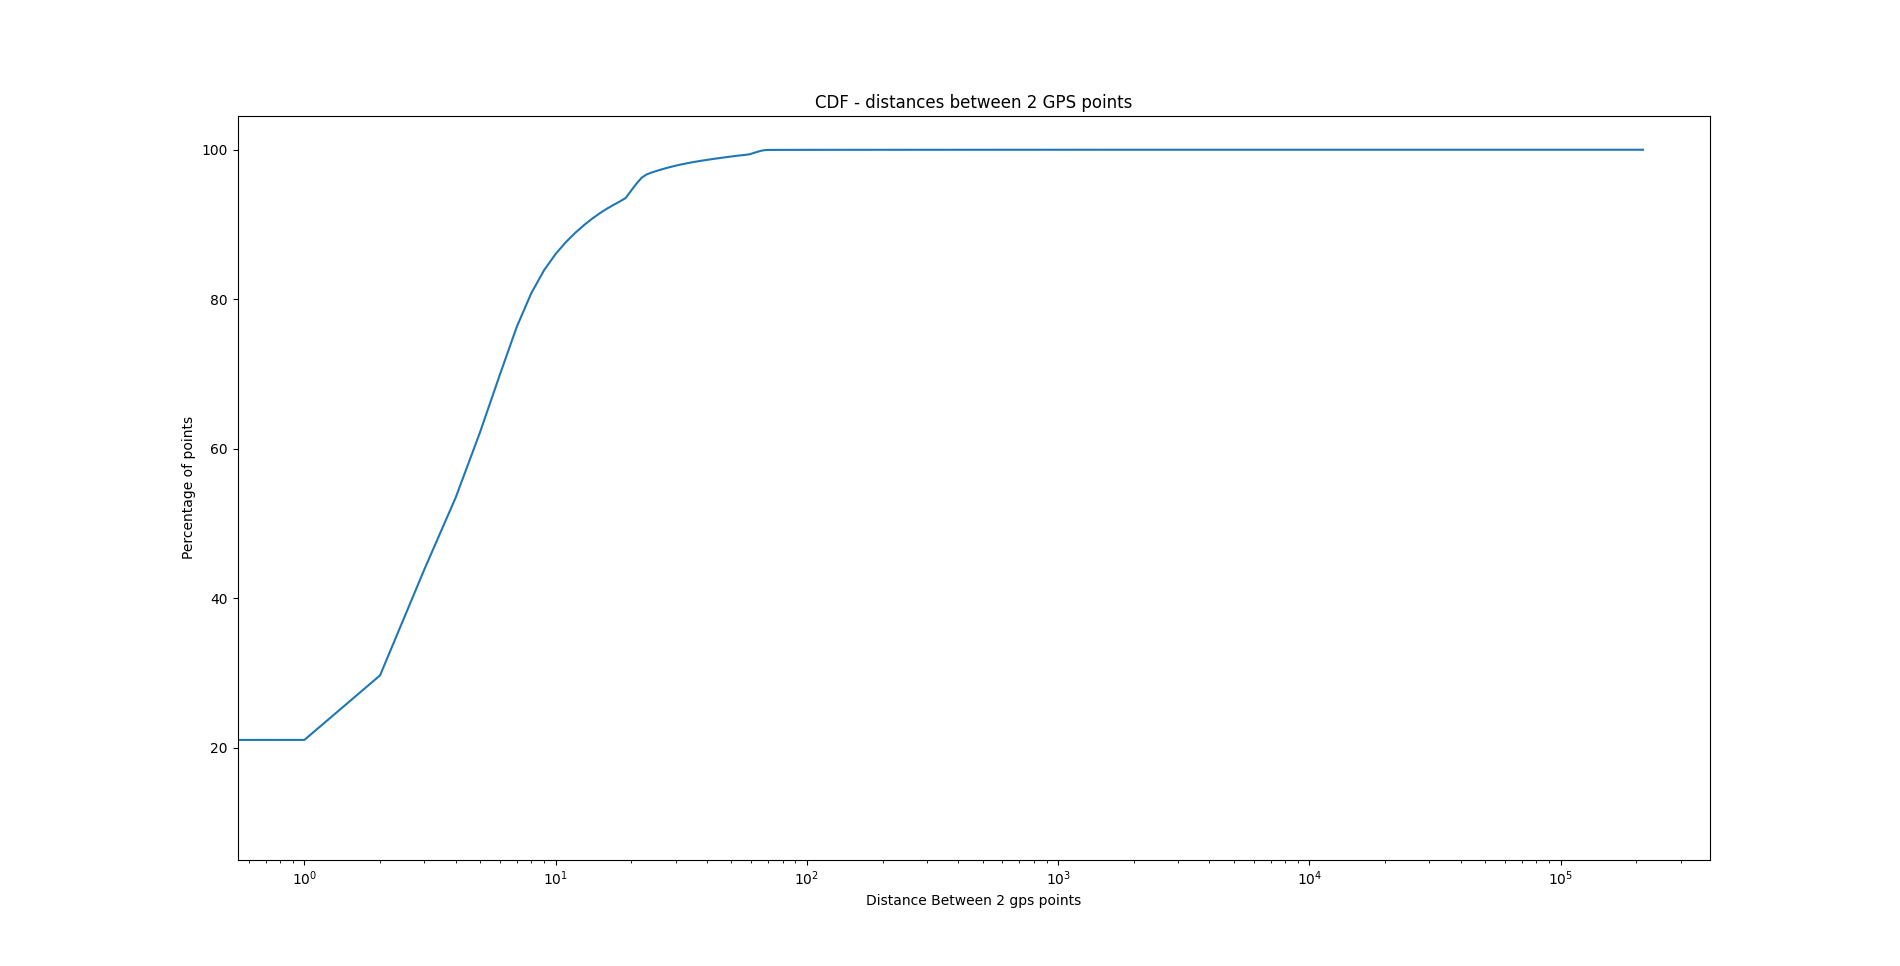
\includegraphics[width=\linewidth]{fig/Afwijkingen&Analyses/Graphs/Afstand tussen 2 gps-punten.png}
    \caption{Distribution of distances between two consecutive GPS points}\label{fig:distance_between_gps_points_CDF}
\end{figure}

To determine the number of GPS deviations in the dataset, we also examine the
difference between the calculated distance traveled within the EPZ (obtained by
subtracting the visible trajectory from the total distance) and the
theoretically traveled distance within the EPZ, which can be read from the
dataset through the cumulative distance. An initial visualization is shown in
Figure~\ref{fig:difference_noCDF}. The figure illustrates the fluctuations
between the manually calculated distance and the theoretical distance for one
user. The peaks indicate significant deviating calculated distances, indicating
large GPS errors. Additionally, the less noticeable fluctuations also indicate
significant inaccuracies between the calculated and theoretical distances. The
differences in calculations for the entire dataset are presented in
Figure~\ref{fig:differences_log}. The graphs reveal that there are indeed many
significant differences present.
\begin{figure}[h]
    \centering
    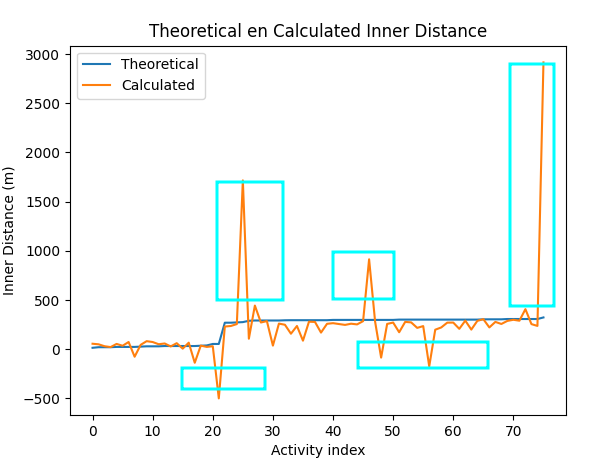
\includegraphics[width=\linewidth]{fig/Afwijkingen&Analyses/Graphs/Verschil_Theoretische_innerDistance.png}
    \caption{Difference between the calculated distance and the theoretical distance for a single user}\label{fig:difference_noCDF}
\end{figure}
\begin{figure}[h]
    \centering
    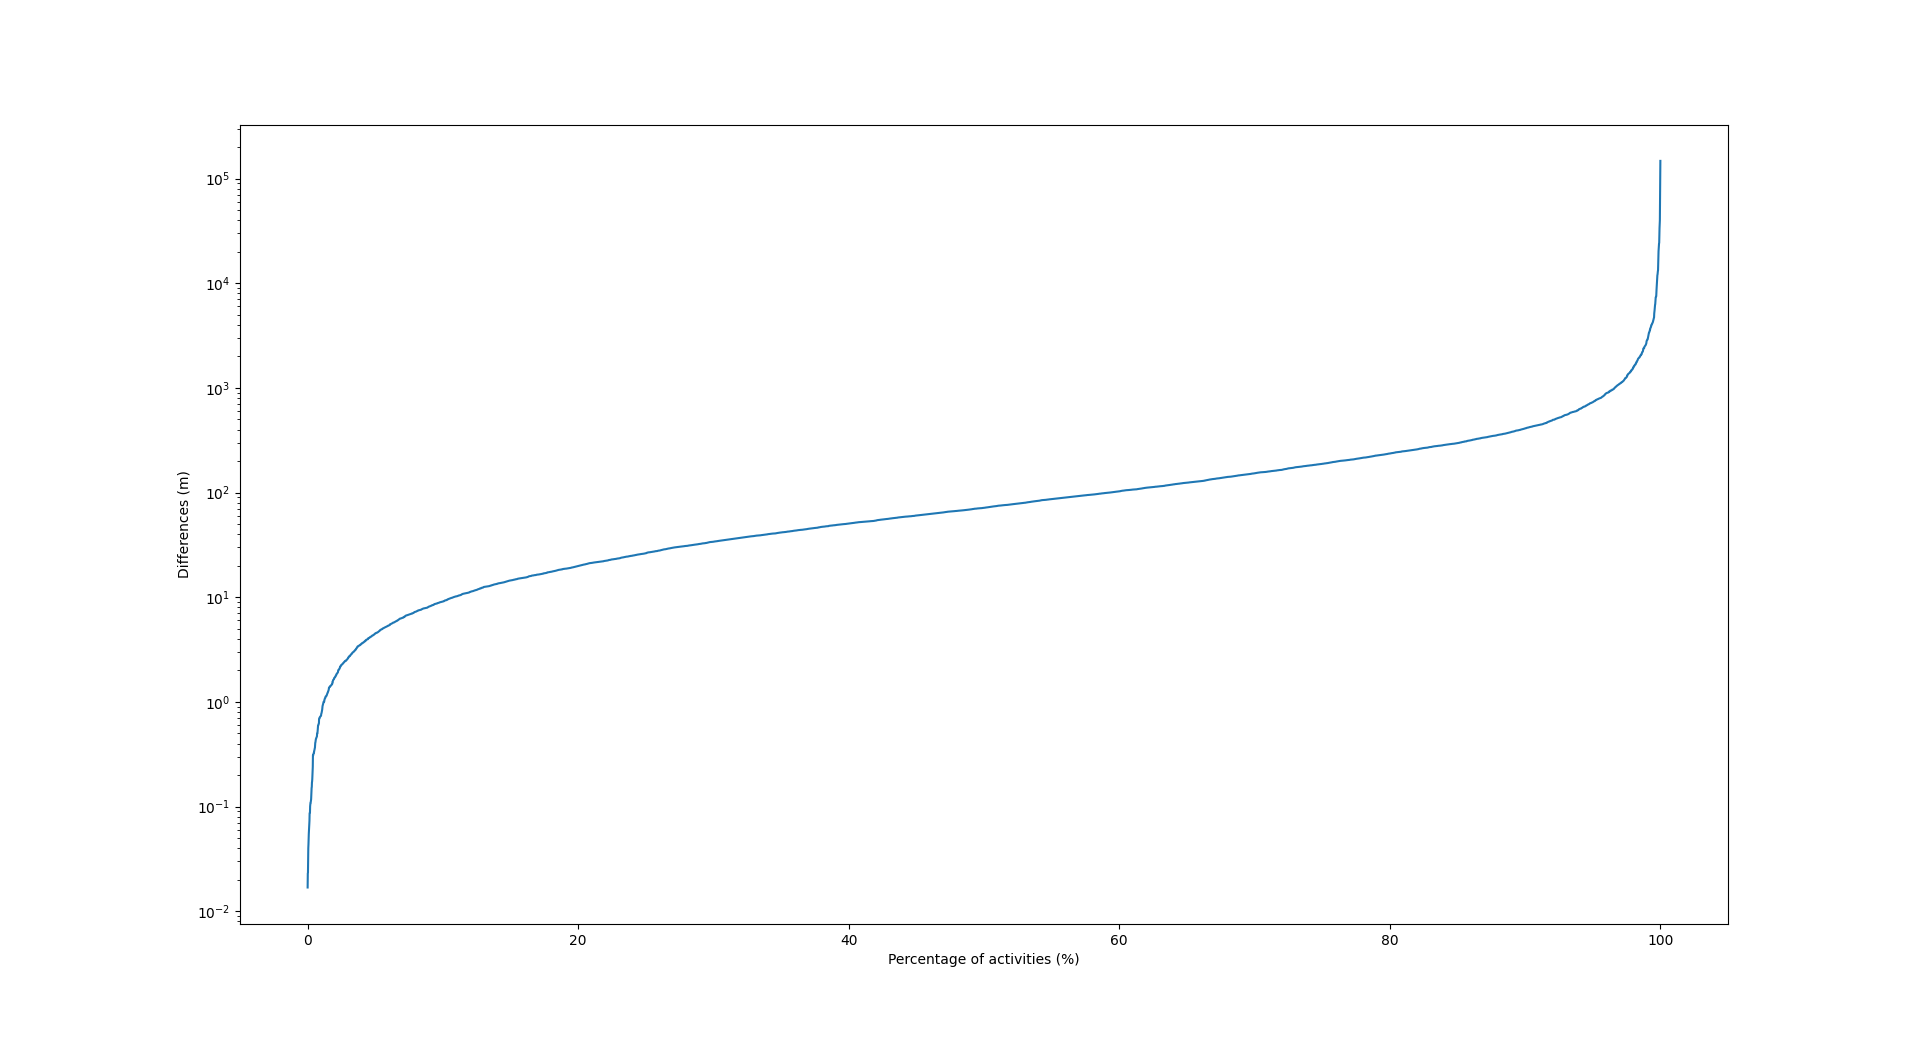
\includegraphics[width=\linewidth]{fig/Afwijkingen&Analyses/Graphs/100_Differences_tov_theoretische_BefSmoothening.png}
    \caption{Distribution of the difference between the calculated distance and the theoretical distance outside the EPZ}\label{fig:differences_log}
\end{figure}

\section{\textbf{Evaluation mechanism}}
We will test and evaluate the attack on public activities that do not contain
an EPZ, but will manually provide them with an EPZ.\ This way, we can compare
the obtained results with a reference, namely the ground truth (GT).

\subsection{ground truth}
The ground truth of a user is their actual place of residence or the location
they typically depart from or arrive at. This is the location we consider as
the center around which the EPZ is applied and the one we ultimately aim to
determine. We determine this location by examining all activities of a user and
adding the starting or ending points that are within a radius of 50 meters to
the same cluster using the DBSCAN algorithm. Please note that it is possible
for a user to have multiple ground truths.

A second caveat we need to mention is that the actual starting and ending
locations may not always align perfectly with the road network. We subsequently
map them to the street network, but during the upload process, the platform in
question calculates the total distance traveled to the actual starting point.
This can introduce deviations in the predictions. Dhondt et al.\ conducted a
study to determine the average deviation and obtained a threshold of 22.95
meters to classify a successful attack~\cite{Dhondt}.

\subsection{Manually adding EPZs}
As mentioned earlier, we are working with public activities that do not contain
an EPZ in order to simplify the evaluation process. However, in order to
perform the attack, we still need to manually introduce an EPZ.\ An EPZ is
determined by a central point (the sensitive location), which will undergo a
random translation, and a chosen radius. From the translated point, a circle is
drawn with the corresponding radius. We start from the ground truth location,
which then undergoes a random translation. The shift of the point can occur in
any direction and is chosen randomly. The distance of the translation can, in
principle, be chosen arbitrarily, but it must fall within certain limits,
namely between 0 and 70\% of the radius of the EPZ.\ The circle is then
constructed with the translated point as the center and the associated radius.
All points within this zone will be removed from the activity.

\subsection{Bootstrapping}
During the testing procedure of the attack, it is not simply performed once for
all activities per user. For each user, a confidence interval is calculated
using bootstrapping. The set of manually obfuscated activities is considered.
The bootstrap algorithm randomly selects one activity at a time from this set
and places it in a new group until this new group of activities is the same
size as the original set of activities. It's important to note that the
algorithm may choose the same activity multiple times, so the newly created
group may contain duplicates and may not include other activities at all. This
process is repeated 1000 times, resulting in 1000 different sets. For each set,
a prediction is made, yielding a number of predicted locations, some of which
may be predicted multiple times.

\subsection{Evaluation metrics}
To provide meaningful insights into the effectiveness of the attack, eight
metrics are defined to evaluate the attack. These metrics are chosen to align
with the metrics used in the studies by Dhondt et al.\ and Verdonck, enabling
clear comparisons with their results~\cite{Dhondt, Verdonck_2022}.

The \textit{Success Rate} is defined as the percentage of performed attacks in
which the sensitive location is successfully determined. Taking into account
the overshoots that may occur when snapping locations to the road network, a
correct location is considered to be within a radius of 22.95 meters from the
ground truth. A higher percentage indicates a more successful attack.

The \textit{Correctness} of an attack is calculated as the sum of the Euclidean
distances between the ground truth and the predicted location, divided by the
number of times that location was predicted. This metric provides an indication
of the average deviation in distance of the predicted locations from the ground
truth. A lower value indicates a more precise attack.

The \textit{Accuracy} in this context is defined as the width of the confidence
interval. It refers to the number of unique predictions, which represents the
number of nodes that are predicted exactly once. A higher number of unique
nodes indicates higher accuracy, but this also implies less certainty in our
predictions.

The \textit{Reduction of the k-anonymity set} quantifies the decrease in the
set of all possible end locations before and after the actual predictions of an
attack. The possible end locations before the attack are simply all nodes in
the graph representation, potentially limited by the EPZ.\ The ones after the
attack are the nodes that are effectively predicted. The reduction is therefore
a percentage that indicates the difference between the two sets. A higher
reduction percentage implies a more significant reduction in the set of
possible end locations, indicating a higher precision of the attack.

The \textit{Uncertainty Region} ($m^2$) is the sum of the areas of the union of
the uncertainty regions around the predicted nodes. In this context, the
uncertainty regions are caused by the chaining distance, which is assumed to be
three meters. Since nodes exist only at intervals of three meters, each
predicted node has a chance of representing a point that lies somewhere within
a three-meter zone around that node. The Uncertainty Region metric quantifies
the combined uncertainty associated with these predicted nodes by calculating
the total area of their uncertainty regions.

The \textit{Certainty metric} quantifies the concentration of the probability
distribution. A higher Certainty value indicates that the nodes in the
probability distribution are spread further apart, indicating a greater level
of certainty or confidence in the predictions. Essentially, it measures the
degree of dispersion or concentration of the predicted locations in the
probability distribution.

\textit{Spatial Certainty} is a metric that considers the density or concentration of
neighboring nodes in the vicinity of each predicted node, instead of focusing
solely on the probability of each individual node. It takes into account the
density or clustering of predicted locations in the neighbourhood of each node.
A higher Spatial Certainty value indicates a higher density or concentration of
predicted nodes in the local vicinity, suggesting a higher level of certainty
in the predicted locations within their respective neighbourhoods.

The \textit{Degree of Anonymity} is a metric that quantifies the level of
anonymity achieved by the attack. It is calculated as the normalized entropy of
the expected distribution, where the entropy represents the amount of
uncertainty or randomness in the distribution of predicted locations. By
normalizing it based on the maximum possible entropy, the Degree of Anonymity
provides a measure of how much information is leaked or preserved by the
attack.

\section{\textbf{Results}}

Each of the four described scenarios will be discussed separately and compared
to each other. The difference in results is visible on
Figure~\ref{fig:attack_comparison}. The individual results are given by the
tables in Appendix~\ref{app:individual_results}. In general, a similar trend is
observed across the models when changing the EPZs. As the radius increases, the
success rate decreases due to the inclusion of more nodes. More nodes lead to
increased potential confusion in the LAD regression. This also results in a
greater degree of anonymity and uncertainty region. The number of predictions
does not increase proportionally with the number of nodes in the graph as the
size expands, leading to an increased reduction. Lastly, it is noticeable that
the correctness also improves with a larger radius. This is attributed to a
higher probability of violating one of the specified assumptions.
\begin{figure}[h]
    \centering
    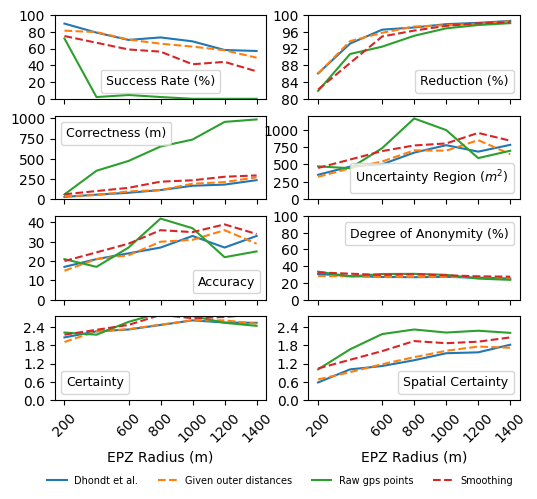
\includegraphics[width=\linewidth]{fig/result_graphs/all_results.png}
    \caption{Comparison of different attack models}\label{fig:attack_comparison}
\end{figure}

\subsection{Model according to Dhondt et al.}
The first model we test is the model by Dhondt et al.~\cite{Dhondt}.We use
these results as a reference for the rest of the findings. The model by Dhondt
et al.\ does not have any restrictions regarding the available data, so it can
utilize all the data. It is therefore expected that this leads to good scores.

\subsection{Given outer distance}
This model is based on the availability of cumulative distances. One advantage
of this model is that it does not require GPS data. We observe a similar trend
as in the model by Dhondt et al., with slight declines in most scores compared
to their results. There is only one additional step necessary compared to the
model by Dhondt et al., which involves converting speed and time to total
distance. This conversion accounts for the minor decreases and increases in the
results. The conversion process may introduce small deviations, likely due to
rounding errors and additional calculations performed by Strava in determining
the speed.

\subsection{Raw GPS data}

The next attack scenario is performed without using cumulative distance and
without smoothing. This means that the attacker directly utilizes the raw GPS
data for calculating the outer distance. In this case, both the deviation
resulting from the speed conversion discussed in the previous model (where the
outer distance is given) and the deviations originating from the GPS data
itself are incorporated in the results.

As expected, these deviations have a relatively strong impact. Especially for
larger radii, they significantly affect the results. From a radius of 1000
meters onwards, the success rate drops to 0\%. We also observe a substantial
decline in the scores of other metrics for higher EPZ radii. This can be
attributed to the significant deviations introduced by the raw GPS data, which
have a particularly noticeable effect at larger radii. The longer the distance
to be traveled, in this case the inner distance, the greater the error.

\subsection{Smoothing}
The final model is similar to the previous one, with the difference that
smoothing is now applied to the routes in an attempt to reduce the deviations
caused by GPS data. Smoothing helps to flatten out the extremes and should
reduce errors to a lower order. This is reflected in the results. The success
rate shows a relatively small improvement compared to the model using raw GPS
data for smaller EPZs, but for larger EPZs, the metrics exhibit much less
deterioration. The other metrics also demonstrate a similar pattern, with the
attenuation being much less pronounced than when using raw GPS points. This
indicates that the use of smoothing provides a significant added value.
However, it's important to note that the optimal smoothing window size was
determined empirically and tailored specifically to this dataset. For a
different dataset, the optimal window size may vary.

\section{\textbf{Conclusion}}

This thesis demonstrates that inference attacks are possible based on speeds
and GPS data, albeit with a lower success rate and increased uncertainty. If
cumulative distance is available, a simple conversion ($inner\ distance =
    total\ time \times average\ speed - outer\ distance \label{eq:inner}$) allows
the attack to be performed with a success rate of up to 81.43\%, which is
deemed acceptable. If cumulative distance data is not available, an additional
conversion can be performed using GPS locations to still achieve a successful
attack. By incorporating smoothing algorithms, the attack can also gain
precision, resulting in a success rate of up to 75.0\% for the respective radii
and a smoothing window of 100. While this success rate is acceptable, it is
lower than the success rate achieved by Dhondt et al. Hence, certain distance
data, specifically cumulative distance and total distance, are not crucial for
the successful execution of this attack model.

Dhondt et al.\ proposed several measures to ensure user privacy, such as
rounding distance data or adding noise to make it unusable~\cite{Dhondt}.
However, our attack model can bypass all the \textit{Distance Focused
    Countermeasures}described by Dhondt et al., except for the Shifting distances
countermeasure. The four distance focused countermeasures are: \begin{itemize}
    \item \textit{Generalization} involves rounding the distance to a certain precision. Dhondt et
          al.\ suggests a precision of 500 meters.
    \item \textit{Noisy Distances} is a technique where a random value is added or subtracted from
          the total distance.
    \item \textit{Shifting Distances} shifts the visible start or end points of an activity by a
          random distance in a random direction, making the starting point uncertain.
    \item \textit{Truncation} states that the hidden segment is not taken into account in the
          total distance. This effectively removes the hidden segment entirely from
          the activity.
\end{itemize}The
attacker can theoretically recompute the distance data and ultimately still
succeed in the attack. In principle, we could expand these countermeasures by
incorporating speed and/or time. For example, in generalization, which involves
rounding a visible distance, the speed can undergo a similar manipulation. By
considering additional factors beyond distance, we can enhance the
effectiveness of privacy countermeasures.

In the case of the other category of countermeasures, namely
\textit{EPZ-Focused Countermeasures}, it is expected that these still remain
effective countermeasures. These countermeasures include: \begin{itemize}
    \item \textit{Increasing EPZ radii}, as the name suggests, involves enlarging the EPZ. We
          observe that the attack performs significantly less effectively with larger EPZ
          radii.
    \item \textit{Complex EPZ shapes} implements an EPZ that  is no longer a simple circle but takes on
          a more intricate form. This can include shapes such as polygons.
\end{itemize}

\section{\textbf{Future work}}
Some interesting future studies could be conducted to further improve the attack.

Implementing road snapping as a first possibility could enhance the accuracy of
location data by snapping GPS points to the nearest road or path. This can help
eliminate outliers and improve the overall quality of the data used in the
attack model.

Using a dynamic window for smoothing is also a valuable addition. By adjusting
the window size based on factors such as the density of GPS points or the speed
of movement, the smoothing algorithm can better adapt to different scenarios
and reduce the impact of outliers or irregularities in the data.

Furthermore, conducting an additional analysis to identify the external
circumstances under which the attack is most successful is a proactive
approach. This analysis can help identify patterns or vulnerabilities that
contribute to the effectiveness of the attack model. By understanding these
factors, appropriate measures can be taken to mitigate the risk and enhance
user privacy in specific contexts or situations.

\bibliographystyle{IEEEtran}
\bibliography{bibliografie_eng}

\onecolumn
\appendix
\subsection{Individual attack results}\label{app:individual_results}
\begin{table*}[h]
    \centering
    \scalebox{0.8}{
        \begin{tabular}{lrrrrrrrr}
            \toprule
            {}         & Success Rate (\%) & Correctness (m) & Accuracy & Reduction (\%) & Uncertainty Region ($m^2$) & Certainty & Spatial Certainty & Degree of Anonymity (\%) \\
            Radius (m) &                   &                 &          &                &                            &           &                   &                          \\
            \midrule
            200        & 89.86             & 28.61           & 17       & 86.06          & 352.08                     & 2.06      & 0.58              & 30.69                    \\
            400        & 79.1              & 56.82           & 21       & 93.21          & 469.76                     & 2.26      & 1.01              & 28.31                    \\
            600        & 70.37             & 79.94           & 24       & 96.52          & 502.42                     & 2.32      & 1.12              & 27.15                    \\
            800        & 73.33             & 113.68          & 27       & 97.05          & 670.53                     & 2.47      & 1.31              & 26.86                    \\
            1000       & 68.64             & 166.74          & 33       & 97.84          & 777.57                     & 2.62      & 1.54              & 27.25                    \\
            1200       & 58.33             & 180.97          & 27       & 98.15          & 684.71                     & 2.55      & 1.57              & 26.25                    \\
            1400       & 57.14             & 235.76          & 33       & 98.61          & 782.30                     & 2.54      & 1.82              & 25.31                    \\
            \bottomrule
        \end{tabular}
    }
    \captionsetup{justification=centering}
    \caption{Attack according to the model by Dhondt et al.~\cite{Dhondt}}\label{tab:aanval_karel}
\end{table*}

\begin{table*}[h]
    \centering
    \scalebox{0.8}{
        \begin{tabular}{lrrrrrrrr}
            \toprule
            {}         & Success Rate (\%) & Correctness (m) & Accuracy & Reduction (\%) & Uncertainty Region ($m^2$) & Certainty & Spatial Certainty & Degree of Anonymity (\%) \\
            Radius (m) &                   &                 &          &                &                            &           &                   &                          \\
            \midrule
            200        & 81.43             & 35.96           & 15       & 86.01          & 322.32                     & 1.91      & 0.68              & 28.33                    \\
            400        & 79.71             & 51.38           & 21       & 93.78          & 445.30                     & 2.26      & 0.92              & 27.80                    \\
            600        & 70.77             & 96.94           & 23       & 95.78          & 542.48                     & 2.33      & 1.18              & 27.34                    \\
            800        & 65.83             & 113.18          & 30       & 97.28          & 703.00                     & 2.48      & 1.41              & 27.38                    \\
            1000       & 62.39             & 191.47          & 31       & 97.60          & 698.69                     & 2.62      & 1.62              & 27.31                    \\
            1200       & 57.98             & 212.06          & 36       & 97.86          & 850.01                     & 2.62      & 1.76              & 27.13                    \\
            1400       & 49.15             & 270.35          & 29       & 98.54          & 648.70                     & 2.51      & 1.72              & 24.90                    \\
            \bottomrule
        \end{tabular}
    }
    \captionsetup{justification=centering}
    \caption{Attack based on given \textit{outer distance}, and speed}\label{tab:outerDistance}
\end{table*}

\begin{table*}[h]
    \centering
    \scalebox{0.8}{
        \begin{tabular}{lrrrrrrrr}
            \toprule
            {}         & Success Rate (\%) & Correctness (m) & Accuracy & Reduction (\%) & Uncertainty Region ($m^2$) & Certainty & Spatial Certainty & Degree of Anonymity (\%) \\
            Radius (m) &                   &                 &          &                &                            &           &                   &                          \\
            \midrule
            200        & 72.06             & 59.92           & 21       & 81.89          & 473.05                     & 2.22      & 1.01              & 33.43                    \\
            400        & 2.08              & 351.85          & 17       & 90.71          & 446.35                     & 2.15      & 1.67              & 27.80                    \\
            600        & 4.55              & 473.15          & 27       & 92.46          & 734.62                     & 2.57      & 2.17              & 30.67                    \\
            800        & 2.13              & 651.38          & 42       & 95.06          & 1161.95                    & 2.87      & 2.32              & 30.84                    \\
            1000       & 0.00              & 737.93          & 37       & 96.84          & 994.80                     & 2.76      & 2.22              & 29.69                    \\
            1200       & 0.00              & 955.79          & 22       & 97.63          & 592.09                     & 2.54      & 2.28              & 25.16                    \\
            1400       & 0.00              & 986.46          & 25       & 98.08          & 697.50                     & 2.44      & 2.21              & 23.70                    \\
            \bottomrule
        \end{tabular}
    }
    \captionsetup{justification=centering}
    \caption{Attack based on raw GPS locations (no smoothing) and speed}\label{tab:noSmoothing}
\end{table*}

\begin{table*}[h]
    \centering
    \scalebox{0.7}{
        \begin{tabular}{lrrrrrrrrr}
            \toprule
            {}         &                      & Success Rate (\%) & Correctness (m) & Accuracy & Reduction (\%) & Uncertainty Region ($m^2$) & Certainty & Spatial Certainty & Degree of Anonymity (\%) \\
            Radius (m) & Smoothing Window (n) &                   &                 &          &                &                            &           &                   &                          \\
            \midrule
            200        & 100                  & 75.0              & 61.37           & 20       & 82.22          & 450.15                     & 2.15      & 1.04              & 32.57                    \\
            600        & 100                  & 58.97             & 141.04          & 29       & 94.89          & 692.52                     & 2.47      & 1.61              & 29.51                    \\
            800        & 100                  & 56.34             & 217.13          & 36       & 96.30          & 773.61                     & 2.80      & 1.94              & 30.30                    \\
            1000       & 100                  & 41.27             & 234.27          & 35       & 97.43          & 802.93                     & 2.69      & 1.87              & 29.13                    \\
            1200       & 100                  & 44.12             & 278.00          & 39       & 98.06          & 953.93                     & 2.73      & 1.92              & 27.86                    \\
            1400       & 100                  & 32.81             & 294.24          & 34       & 98.28          & 841.94                     & 2.82      & 2.06              & 27.51                    \\
            \bottomrule
        \end{tabular}
    }
    \captionsetup{justification=centering}
    \caption{Attack based on smoothed GPS data and velocity, with an empirically determined optimal smoothing window $n=100$}\label{tab:optimal_smoothing}
\end{table*}

\end{document}